\chapter{Introduction} 

In statistics, we come across various collections of probability distributions, such as the normal distribution, Poisson distribution, and binomial distribution. These distributions are used to model random variables in applications and are referred to as \emph{statistical models}. Precisely, a statistical model is just a set of probability distributions. If the set contains only discrete distributions, we call it a \emph{discrete statistical model}. In this case, discrete statistical models are just subsets of the probability simplex \( \Delta_n \coloneqq \left\{ p \in \mathbb{R}^{n + 1} \mid \sum p_i = 1 \right\} \). 

A discrete distribution \( p \in \mathcal{M} \subset \Delta_n \) from a discrete statistical model encapsulates the probabilities of observing the states \( 0, \dots, n \), i.e. if \( X \in \left\{ 0, \dots, n \right\} \) is a discrete random variable, then the state \( X = i \) occurs with probability \( p_i \) for all \( i = 0, \dots, n \). Say we have a binomial random variable \( X \) with \( n + 1 \) states, then \( p_i = \binom{n}{i} \theta^i (1-\theta)^{n-i} \) computes the probability of observing \( i \) successes in \( n \) trials with success probability \( \theta \in [0,1] \). The set \( \mathcal{M} \) of all probability distributions of that form, i.e. \( \mathcal{M} = \left\{ (\binom{n}{i} \theta^i (1-\theta)^{n-i})_{i=0}^n \mid \theta \in [0,1] \right\} \), is our first example of a discrete statistical model, and is known as the \emph{binomial model}.

\begin{figure}
    \centering
    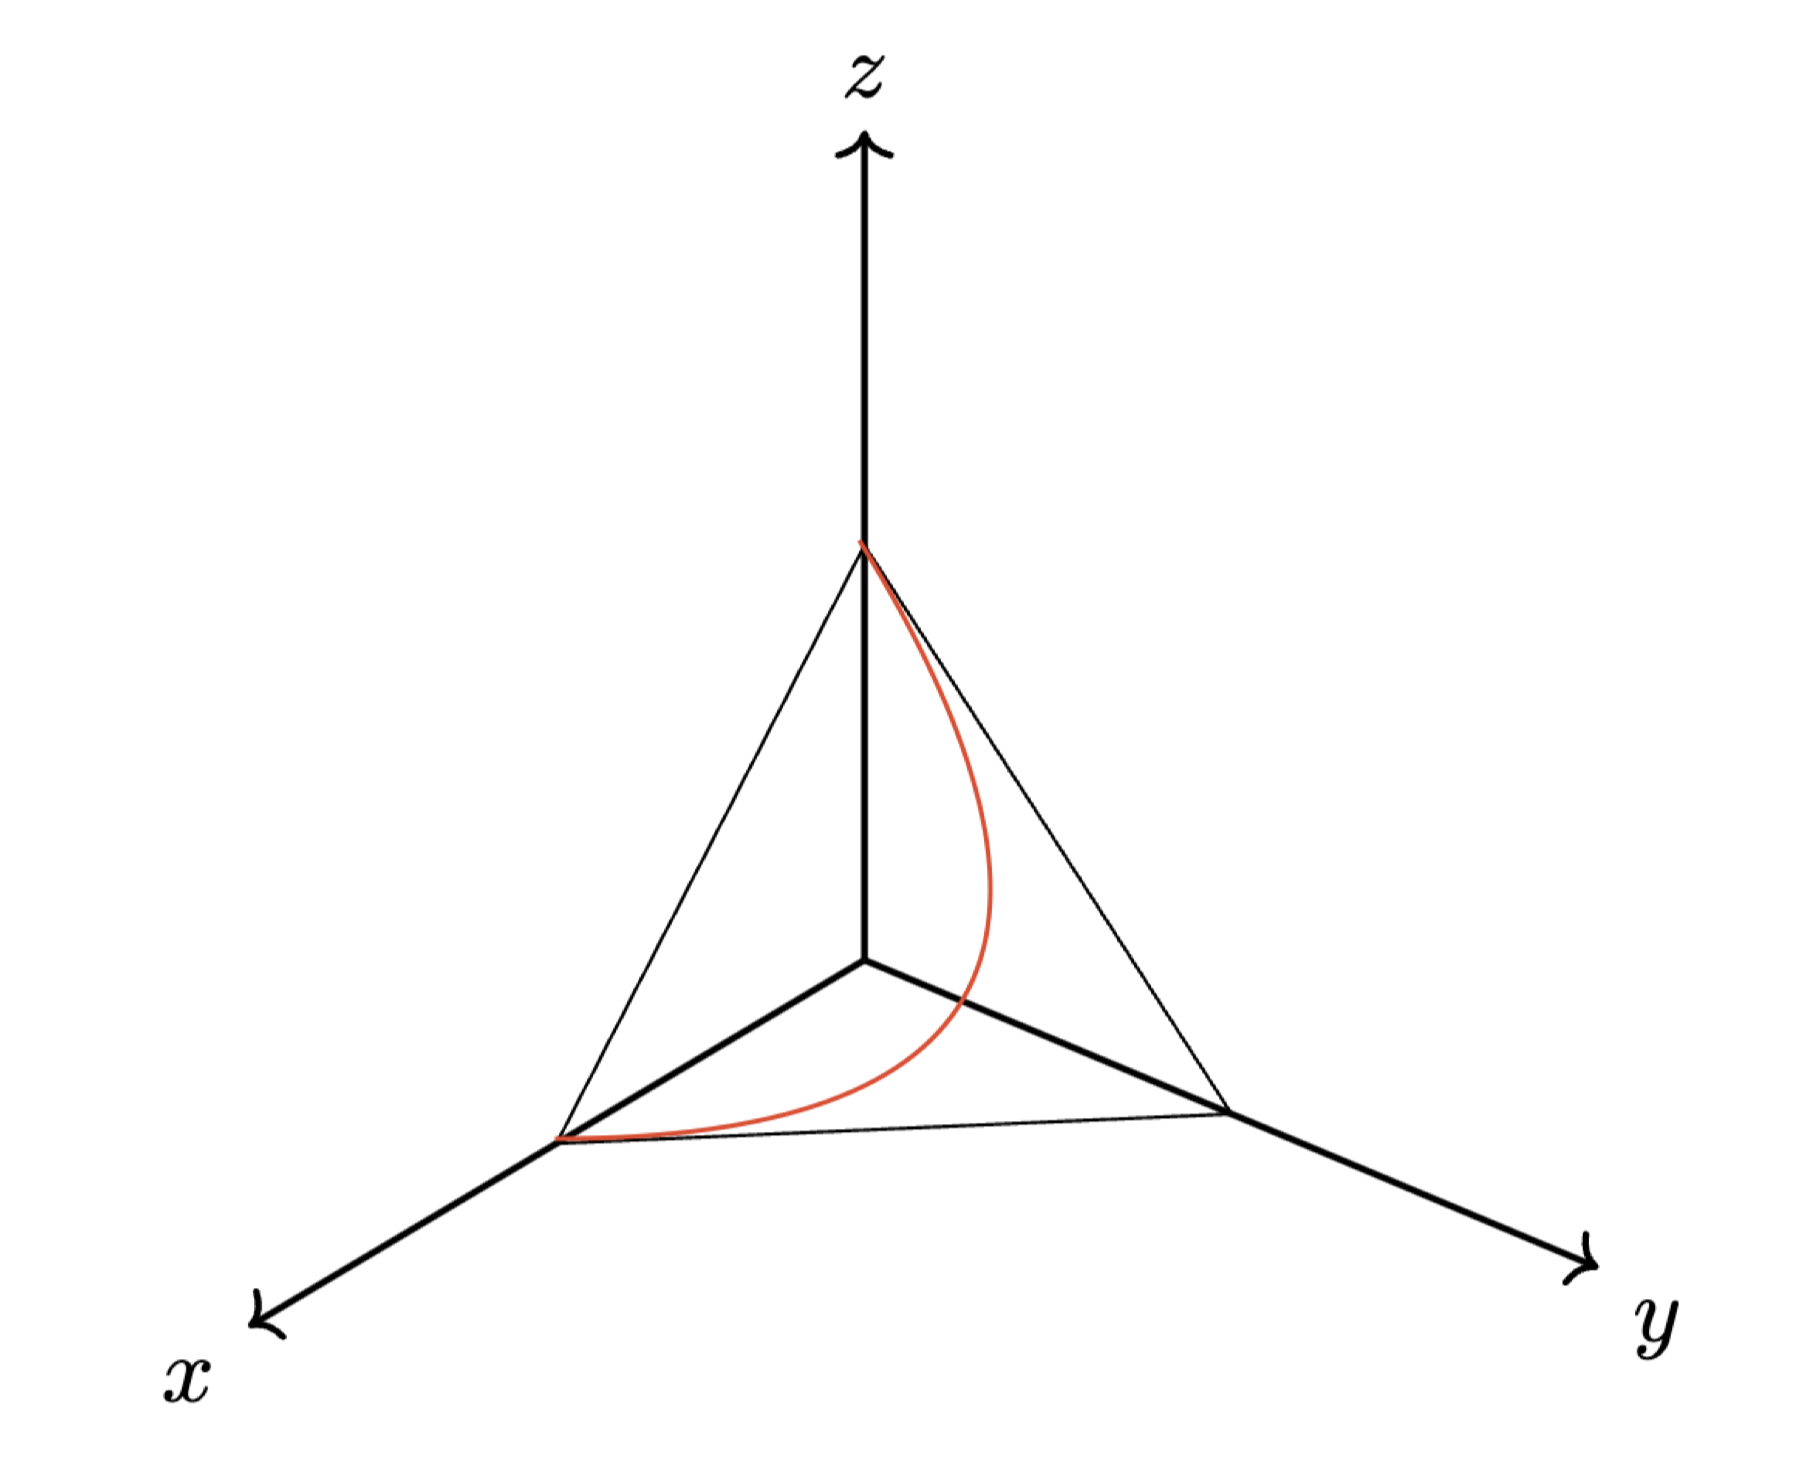
\includegraphics[width=0.4\textwidth]{assets/binom-discrete-model.png}
    \caption{This figure shows the probability simplex \( \Delta_2 \) with the binomial model (red curve). Every point on the curve is a binomial distribution.}
    \label{fig:binom-discrete-model}
\end{figure}

Given a statistical model \( \mathcal{M} \subset \Delta_n \) and data \( u \in \mathbb{N}^{n+1} \), a typical problem in statistics is to find a distribution from a statistical model that best describes the data. ``Best'' can mean a lot of things, but in \emph{maximum likelihood estimation} it means finding the distribution that maximizes the probability of observing the data; the map \( \Phi: \Delta_n \to \mathcal{M}, u \mapsto \hat p \) that assigns the data \( u \) to a distribution \( \hat p \in \mathcal{M}\) from the statistical model is called the \emph{maximum likelihood estimator (MLE)}. This map is characterized by the property that \( \hat p \) maximizes the log-likelihood function \( \ell(p) = \sum u_i \log p_i \) for all \( p \in \mathcal{M} \). 

We focus on \textbf{{one-dimensional {discrete} {statistical} {models} with rational MLE}}. These are models \( \mathcal{M} \) satisfying 
\begin{itemize}
    \item \( \mathcal{M} = \mathrm{image}(p) \) for some rational map \( p = (p_0, \dots, p_n): I \to \Delta_n \) where \( p_i \) is rational, \( I \subset \mathbb{R} \) is a union of closed intervals and  \( p(\partial I) \subset \partial \Delta_n \),
    \item all the \( n+1 \) coordinates of the maximum likelihood estimator \( \Phi \) are rational functions in the data \( u \).
\end{itemize}
There are two intriguing questions to ask about statistical models with rational MLE: the first one is about which \emph{form} they take; the second one is more concerned with the \emph{classification} of the statistical models, i.e. can we divide these models into easier to understand classes? An answer to the first question was given by June Huh. He showed that if \( \Phi \) is rational, then each of its coordinates is an alternating product of linear forms with a numerator and denominator of the same degree, see \cite{huh2013varieties, huh2013maximum, duarte2021discrete}. For the second question, Arthur Bik and Orlando Marigliano classified all one-dimensional discrete statistical models with rational MLE using \emph{fundamental models} \cite{bik2022classifying}.

This thesis continues the work of Bik and Marigliano. In the first half, we present their classification results on how fundamental models serve as the building blocks of one-dimensional discrete models with rational MLE. In the second half, we establish and extend their finding that there are only finitely many fundamental models within the probability simplices \( \Delta_n  \) for \( n \leq 4 \). Due to the complexity of the problem, the cases \( n \geq 5 \) were left open. We make progress for \( n = 5 \) by reducing the number of cases to check from 300,000 to 12,000. Additionally, this thesis introduces new results on the number of fundamental models in \( \Delta_6 \), with a maximum degree of eleven, and provides an algorithm for solving non-trivial hyperfield linear systems, which is essential to all the computational work presented.

The outline of this thesis is as follows: 
\begin{itemize}
    \item Chapter 2 provides a classification of statistical models using fundamental models.
    \item Chapter 3 introduces chipsplitting games and establishes the connection to fundamental models via chipsplitting outcomes.
    \item Chapter 4 develops the \emph{Invertibility Criterion}, and Chapter 5 applies it.
    \item Chapter 6 introduces the \emph{Hyperfield Criterion}, and Chapter 7 uses these tools to establish a bound on the degree for positive support size four outcomes.
    \item Chapter 8 introduces the final tool, the Hexagon Criterion, to tackle outcomes with positive support size five, and Chapter 9 applies it.
    \item Chapter 10 presents new techniques to reduce the number of cases that need to be analyzed to prove that the degree of valid outcomes with support size six is bounded.
    \item Chapter 11 computes the number of fundamental outcomes.
    \item Chapter 12 concludes with a discussion on future research directions and the implications of the findings.
\end{itemize}


The source code for the computations discussed in this thesis is available at \cite{ducrepo}.
